\section{Git and GitHub}
In this project, we used GitHub to host our report LaTeX code, and the source code for our flutter application.
We have used Git to interact with GitHub and push and pull code. 

GitHub is also linked to our Azure Pipelines as described in~\autoref{azurepipelines}.

We use the principles of Gitflow, that requires developers to create a branch for each new feature, hot fixes and bug fixes. 
The branches can then be merged back into their respective branches when the branch is completed.
This is done using pull requests, which has to be approved by at least one other developer.
This ensures that no code is merged into the main branches, with approval of at least one other developer.

\begin{figure}[H]
    \centering
    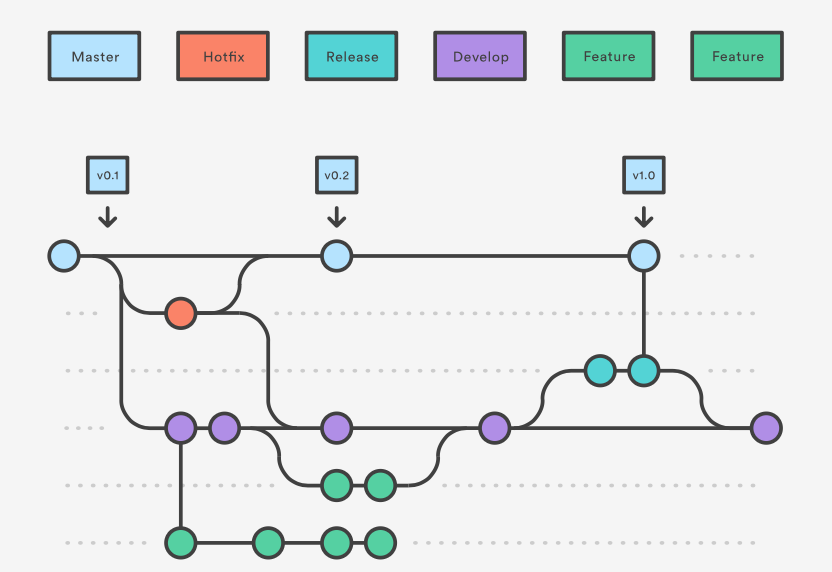
\includegraphics[width=0.8\textwidth]{images/GitFlow.png}
    \caption{Gitflow diagram, showing how branches should be created and named.}
    \label{Gitflow}
\end{figure}
